
\documentclass{standalone}
\usepackage[T1]{fontenc}\usepackage{tikz}
\usepackage{amsmath, amsfonts}
\usetikzlibrary{arrows.meta}
\begin{document}
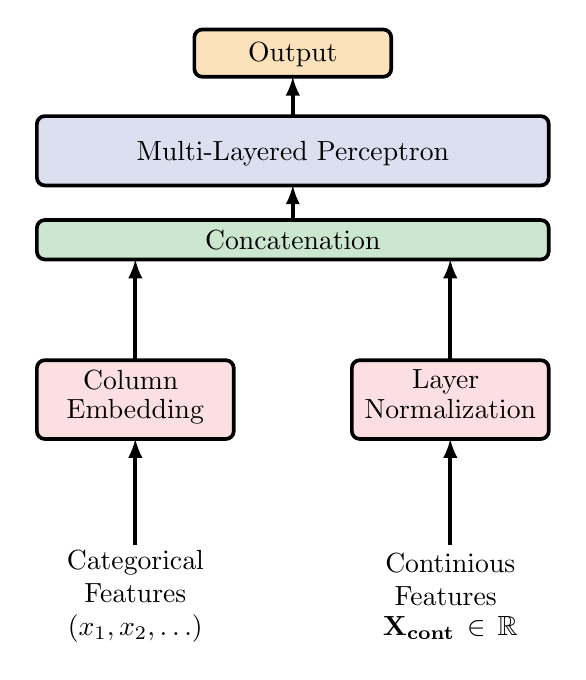
\begin{tikzpicture}
\definecolor{emb_color}{RGB}{252,224,225}
\definecolor{multi_head_attention_color}{RGB}{252,226,187}
\definecolor{add_norm_color}{RGB}{242,243,193}
\definecolor{ff_color}{RGB}{194,232,247}
\definecolor{softmax_color}{RGB}{203,231,207}
\definecolor{linear_color}{RGB}{220,223,240}
\definecolor{gray_bbox_color}{RGB}{243,243,244}

\draw[line width=0.046875cm, fill=multi_head_attention_color, rounded corners=0.100000cm] (2.0, 12.70000) -- (4.500000, 12.7) -- (4.500000, 12.10000) -- (2.0, 12.1) -- cycle;
\node[text width=2.500000cm, anchor=south, align=center] at (3.250000,12.10000) {Output};

\draw[line width=0.046875cm, fill=linear_color, rounded corners=0.100000cm] (0.0, 11.60000) -- (6.500000, 11.6) -- (6.500000, 10.720000) -- (0.000000, 10.720000) -- cycle;
\node[text width=5.00000cm,  align=center] at (3.25,11.130000) {Multi-Layered Perceptron};

\draw[line width=0.046875cm, fill=softmax_color, rounded corners=0.100000cm] (0.0, 10.280000) -- (6.500000, 10.28) -- (6.500000, 9.780000) -- (0.000000, 9.780000) -- cycle;
\node[text width=5.00000cm,  align=center] at (3.25,10.030000) {Concatenation};

\draw[line width=0.046875cm, fill=emb_color, rounded corners=0.100000cm] (0.000000, 8.500000) -- (2.500000, 8.500000) -- (2.500000, 7.50000) -- (0.000000, 7.50000) -- cycle;
\node[text width=2.500000cm, anchor=north, align=center] at (1.250000,8.500000) {Column \vspace{-0.05cm} \linebreak Embedding};


\draw[line width=0.046875cm, fill=emb_color, rounded corners=0.100000cm] (4.000000, 8.500000) -- (6.500000, 8.500000) -- (6.500000, 7.50000) -- (4.000000, 7.5000) -- cycle;
\node[text width=2.500000cm, anchor=north, align=center] at (5.250000,8.500000) {Layer \vspace{-0.05cm} \linebreak Normalization};


\node[text width=2.500000cm, align=center] at (1.250000,5.50000) {Categorical Features \linebreak $(x_1, x_2, \hdots)$};
\node[text width=2.500000cm, align=center] at (5.250000,5.5) {Continious Features \vspace{-0.05cm} \linebreak $\bf{X}_{cont} \in \mathbb{R}$};


\draw[line width=0.046875cm, -latex] (1.250000, 6.15) -- (1.250000, 7.50);
\draw[line width=0.046875cm, -latex] (1.250000, 8.5) -- (1.250000, 9.78);

\draw[line width=0.046875cm, -latex] (5.250000, 6.15) -- (5.250000, 7.50);
\draw[line width=0.046875cm, -latex] (5.250000, 8.5) -- (5.250000, 9.78);

\draw[line width=0.046875cm, -latex] (3.25, 10.28) -- (3.25, 10.72);
\draw[line width=0.046875cm, -latex] (3.25, 11.6) -- (3.25, 12.1);

\end{tikzpicture}
\end{document}